%%%%%%%%%%%%%%%%%%%%%%%%%%%%%%%%%%%%%%%%%
% UTN BA - Argentina
% Medidas Electrónicas II
% 16/12/18
%
% %%%%%%%%%%%%%%%%%%%%%%%%%%%%%%%%%%%%%%%
%
% Copyright
%
% This template was downloaded from:
% http://www.LaTeXTemplates.com
%
% Original Authors:
% Vel (vel@LaTeXTemplates.com)
% Frits Wenneker
%
% License:
% CC BY-NC-SA 3.0 (http://creativecommons.org/licenses/by-nc-sa/3.0/)
%
%%%%%%%%%%%%%%%%%%%%%%%%%%%%%%%%%%%%%%%%%

%----------------------------------------------------------------------------------------
%	PACKAGES AND OTHER DOCUMENT CONFIGURATIONS
%----------------------------------------------------------------------------------------

%!TeX spellcheck = es-ES

% 10pt font size (11 and 12 also possible), A4 paper (letterpaper for US letter) and two column layout (remove for one column)
\documentclass[10pt, a4paper, twocolumn]{article}

% Specifies the document structure and loads requires packages
%%%%%%%%%%%%%%%%%%%%%%%%%%%%%%%%%%%%%%%%%
% Wenneker Article
% Structure Specification File
% Version 1.0 (28/2/17)
%
% This file originates from:
% http://www.LaTeXTemplates.com
%
% Authors:
% Frits Wenneker
% Vel (vel@LaTeXTemplates.com)
%
% License:
% CC BY-NC-SA 3.0 (http://creativecommons.org/licenses/by-nc-sa/3.0/)
%
%%%%%%%%%%%%%%%%%%%%%%%%%%%%%%%%%%%%%%%%%

%----------------------------------------------------------------------------------------
%	PACKAGES AND OTHER DOCUMENT CONFIGURATIONS
%----------------------------------------------------------------------------------------

\usepackage[english]{babel} % English language hyphenation

\usepackage{microtype} % Better typography

\usepackage{amsmath,amsfonts,amsthm} % Math packages for equations

\usepackage[svgnames]{xcolor} % Enabling colors by their 'svgnames'

\usepackage[hang, small, labelfont=bf, up, textfont=it]{caption} % Custom captions under/above tables and figures

\usepackage{booktabs} % Horizontal rules in tables

\usepackage{lastpage} % Used to determine the number of pages in the document (for "Page X of Total")

\usepackage{graphicx} % Required for adding images

\usepackage{enumitem} % Required for customising lists
\setlist{noitemsep} % Remove spacing between bullet/numbered list elements

\usepackage{sectsty} % Enables custom section titles
\allsectionsfont{\usefont{OT1}{phv}{b}{n}} % Change the font of all section commands (Helvetica)

%----------------------------------------------------------------------------------------
%	MARGINS AND SPACING
%----------------------------------------------------------------------------------------

\usepackage{geometry} % Required for adjusting page dimensions

\geometry{
	top=0.5cm, % Top margin
	bottom=1cm, % Bottom margin
	left=2cm, % Left margin
	right=2cm, % Right margin
	includehead, % Include space for a header
	includefoot, % Include space for a footer
	%showframe, % Uncomment to show how the type block is set on the page
}

\setlength{\columnsep}{7mm} % Column separation width

%----------------------------------------------------------------------------------------
%	FONTS
%----------------------------------------------------------------------------------------

\usepackage[T1]{fontenc} % Output font encoding for international characters
\usepackage[utf8]{inputenc} % Required for inputting international characters

\usepackage{XCharter} % Use the XCharter font

%----------------------------------------------------------------------------------------
%	HEADERS AND FOOTERS
%----------------------------------------------------------------------------------------

\usepackage{fancyhdr} % Needed to define custom headers/footers
\pagestyle{fancy} % Enables the custom headers/footers

\renewcommand{\headrulewidth}{0.0pt} % No header rule
\renewcommand{\footrulewidth}{0.4pt} % Thin footer rule

\renewcommand{\sectionmark}[1]{\markboth{#1}{}} % Removes the section number from the header when \leftmark is used

%\nouppercase\leftmark % Add this to one of the lines below if you want a section title in the header/footer

% Headers
\lhead{} % Left header
%\chead{\textit{\thetitle}} % Center header - currently printing the article title
\rhead{} % Right header

% Footers
\lfoot{} % Left footer
\cfoot{} % Center footer
\rfoot{\footnotesize Page \thepage\ of \pageref{LastPage}} % Right footer, "Page 1 of 2"

\fancypagestyle{firstpage}{ % Page style for the first page with the title
	\fancyhf{}
	\renewcommand{\footrulewidth}{0pt} % Suppress footer rule
}

%----------------------------------------------------------------------------------------
%	TITLE SECTION
%----------------------------------------------------------------------------------------

\newcommand{\authorstyle}[1]{{\large\usefont{OT1}{phv}{b}{n}\color{DarkRed}#1}} % Authors style (Helvetica)

\newcommand{\institution}[1]{{\footnotesize\usefont{OT1}{phv}{m}{sl}\color{Black}#1}} % Institutions style (Helvetica)

\usepackage{titling} % Allows custom title configuration

\newcommand{\HorRule}{\color{DarkGoldenrod}\rule{\linewidth}{1pt}} % Defines the gold horizontal rule around the title

\pretitle{
	\vspace{-30pt} % Move the entire title section up
	\HorRule\vspace{10pt} % Horizontal rule before the title
	\fontsize{32}{36}\usefont{OT1}{phv}{b}{n}\selectfont % Helvetica
	\color{DarkRed} % Text colour for the title and author(s)
}

\posttitle{\par\vskip 15pt} % Whitespace under the title

\preauthor{} % Anything that will appear before \author is printed

\postauthor{ % Anything that will appear after \author is printed
	\vspace{10pt} % Space before the rule
	\par\HorRule % Horizontal rule after the title
	\vspace{20pt} % Space after the title section
}

%----------------------------------------------------------------------------------------
%	ABSTRACT
%----------------------------------------------------------------------------------------

\usepackage{lettrine} % Package to accentuate the first letter of the text (lettrine)
\usepackage{fix-cm}	% Fixes the height of the lettrine

\newcommand{\initial}[1]{ % Defines the command and style for the lettrine
	\lettrine[lines=3,findent=4pt,nindent=0pt]{% Lettrine takes up 3 lines, the text to the right of it is indented 4pt and further indenting of lines 2+ is stopped
		\color{DarkGoldenrod}% Lettrine colour
		{#1}% The letter
	}{}%
}

\usepackage{xstring} % Required for string manipulation

\newcommand{\lettrineabstract}[1]{
	\StrLeft{#1}{1}[\firstletter] % Capture the first letter of the abstract for the lettrine
	\initial{\firstletter}\textbf{\StrGobbleLeft{#1}{1}} % Print the abstract with the first letter as a lettrine and the rest in bold
}

%----------------------------------------------------------------------------------------
%	BIBLIOGRAPHY
%----------------------------------------------------------------------------------------
\bibliographystyle{alpha}

\usepackage{amsmath}
\usepackage{empheq}

%----------------------------------------------------------------------------------------
%	ARTICLE INFORMATION
%----------------------------------------------------------------------------------------

% The article title
\title{
Parámetros S On-Wafer \large\newline\newline
Medidas Electrónicas II
	  }
%Medidas Electrónicas II
\author{
	\authorstyle{Luis Pablo Seva\textsuperscript{1}, Bruno Giuliano Errasti\textsuperscript{1} y Pablo Andrés Di Sabato\textsuperscript{1}} % Authors
	\newline\newline
	\textsuperscript{1}\institution{Universidad Tecnológica Nacional, Ciudad Autónoma de Buenos Aires, Argentina}
}

% Example of a one line author/institution relationship
%\author{\newauthor{John Marston} \newinstitution{Universidad Nacional Autónoma de México, Mexico City, Mexico}}

% ## Date ##
% Add a date here if you would like one to appear underneath the title block, use \today for the current date, leave empty for no date
\date{30 de Noviembre de 2018}

%----------------------------------------------------------------------------------------

\begin{document}

% Print the title
\maketitle

% Apply the page style for the first page (no headers and footers)
\thispagestyle{firstpage}

%----------------------------------------------------------------------------------------
%	ABSTRACT
%----------------------------------------------------------------------------------------

\lettrineabstract{Durante el presente proyecto se realizaron mediciones de parámetros S en un atenuador de 3dB. Esto permitió obtener sus características y gráficas, pudiendo así realizar comparaciones con las especificaciones del fabricante. El proyecto también abarcó realizar correcciones en las mediciones utilizando el software Metas VNA Tools.}

%----------------------------------------------------------------------------------------
%	ARTICLE CONTENTS
%----------------------------------------------------------------------------------------

\section{Introducción}

Para realizar las mediciones se utilizó el atenuador de Analog Devices HMC652LP2E \cite{attenuator}. El proyecto se segmentó en varios procesos, los cuales van a ser descriptas en detalle en secciones y sub-secciones siguientes:

\begin{itemize}
	\item Elección del DUT.
	\item Elección de PCB (teniendo en cuenta características de RF).
	\item Diseño de PCB y estándares de calibración.
	\item Fabricación de PCB.
	\item Mediciones.
	\item Conclusiones.
\end{itemize}

Pueden distinguirse en el proyecto tres grandes etapas o conjuntos de tareas:
\begin{description}
	\item[Etapa diseño] Comprende la selección de componentes y diseño de PCB.
	\item[Etapa Fabricación] Fabricación del PCB y montado del Kit.
	\item[Etapa Medición y conclusiones] Adquisición de datos, mediciones y conclusiones.
\end{description}

%------------------------------------------------

\subsection{Atenuador 3dB AD HMC652LP2E}

El DUT seleccionado es un atenuador de 3dB. Sus principales características son
un ancho de banda de 25Ghz y manejo de potencias de hasta +25dBm. Está preparado
para trabajar en configuración CPW \cite{cpw}, que fue la elegida para realizar la placa de
calibración.

\begin{figure}[hbt!]
	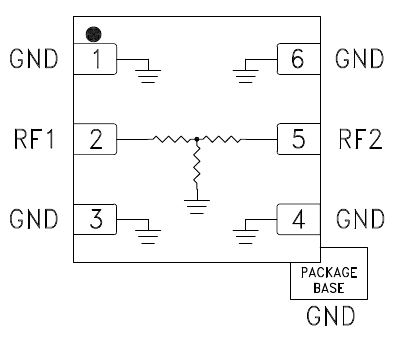
\includegraphics[width=\linewidth]{Fotos/DUT.png}
	\caption{Analog Devices HMC652LP2E.}
\end{figure}

%------------------------------------------------

\subsection{Elección de PCB}

Para la elección del PCB se necesitaban cumplir con ciertos requerimientos y
consideraciones de diseño:
\begin{itemize}
	\item CPW (coplanar waveguide) \cite{cpw}.
	\item Dieléctrico 10.2
	\item Gap y Width limitados, por las características de las puntas de medición (probes): pitch desde 50 a 1250 um.
	\item Conductor de cobre.
\end{itemize}

Teniendo en cuenta todas estas características se optó por elegir un producto de
Rogers Corporation, \textbf{RO3210 Series}\cite{rogers}. Dicho producto cumplía con los requisitos necesarios para el diseño y adicionalmente aplicaba para ser enviado en forma gratuita (fines universitarios). El producto es confeccionado utilizando laminados de cerámica reforzados con fibra de vidrio tejida. Otras características destacadas del producto son
un buen balance entre alta performance eléctrica y estabilidad mecánica (generalmente
hay una relación de compromiso) y un \textbf{factor de disipación muy bajo} (0,0027). Dicha
característica es muy apreciada en el ámbito de RF y particularmente en el presente proyecto
(minimizando pérdidas y errores de medición).

Para realizar los cálculos en base a los requerimientos se utilizó el Software
TX Line \cite{txline}, desarrollado por National Instruments.

\begin{figure}[hbt!]
	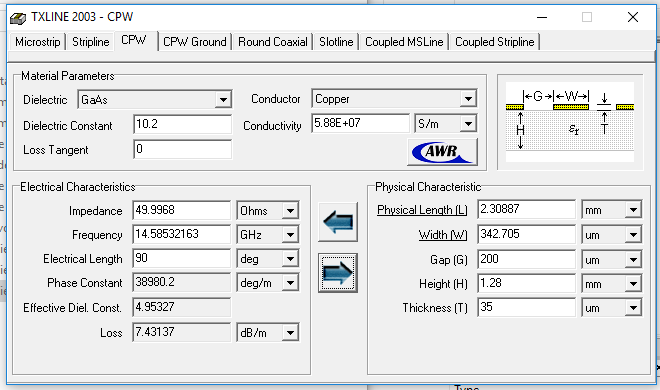
\includegraphics[width=\linewidth]{Fotos/TXLine.png}
	\caption{Validando parámetros con TX Line Software.}
\end{figure}

%------------------------------------------------
\subsection{Diseño y fabricación}

Se diseñó el PCB en base a los requerimientos y cálculos realizados previamente.
Para realizar el layout utilizamos software de diseño CAD (AutoCAD).

\begin{figure}[hbt!]
	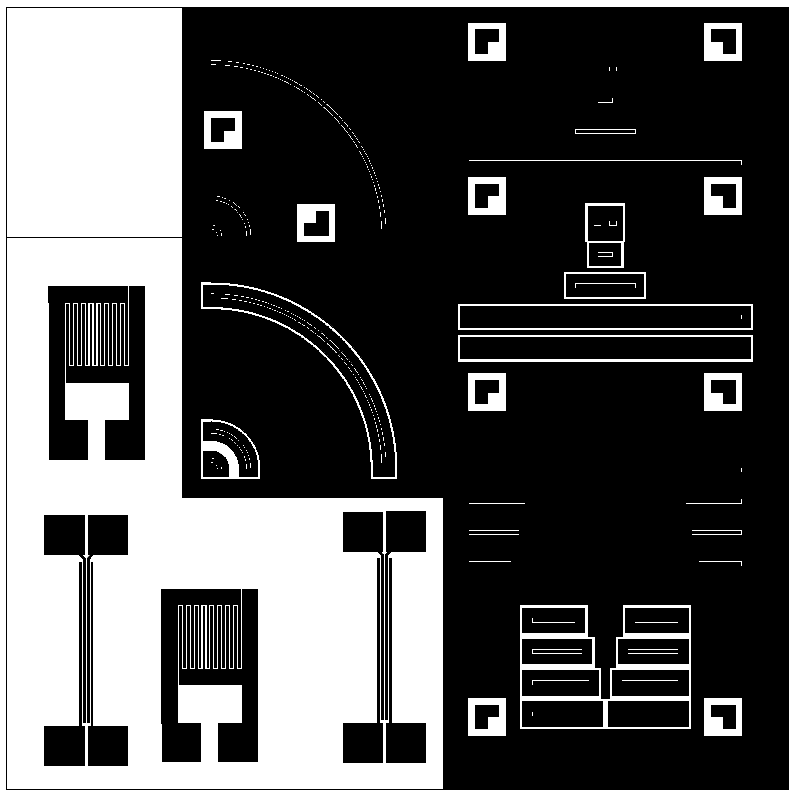
\includegraphics[width=\linewidth]{Fotos/pcb.png}
	\caption{Vista del diseño.}
\end{figure}

Para la fabricación se realizaron dos versiones, una utilizando procesos de fotolitografía
y otra utilizando CNC. Ambas versiones fueron fabricadas en las instalaciones del INTI.

%------------------------------------------------
\section{TRL}
\textbf{TRL (Thru, Reflect, Line)} es una familia de técnicas de calibración que
miden dos patrones de transmisión y uno de reflexión para determinar los
coeficientes de error (2 puertos – 12 términos). Incluyen: TRM (Thru, Reflect, Match), LRL (Line, Reflect, Line) y LRM (Line, Reflect, Match). Se utilizó este método por diversas
características favorables:
\begin{itemize}
\item Excelente precisión.
\item Muy utilizado cuando no se cuenta con patrones de calibración con los mismos tipos de conectores que el DUT (por ejemplo mediciones on-wafer).
\item Utilizado generalmente para realizar mediciones con probe stations.
\item Relativamente sencillo de fabricar e implementar.
\item Los patrones no necesitan ser definidos con tanta precisión y exactitud, ya que son modelados (a diferencia de SOTL).
\end{itemize}

\subsection{Line}

Idealmente, el largo de la pista patrón debe ser exactamente un cuarto de la longitud de onda (90 grados eléctricos). Para realizar un barrido en frecuencia a lo largo de una gran porción del espectro, se vuelve impráctico e irrealizable. Lo más probable es que se requiera realizar mediciones en varias zonas del espectro, por lo que se necesita encontrar un método más apropiado. \newline

Como podemos apreciar, es necesario adoptar ciertos criterios para utilizar el método en
forma práctica. Esto quiere decir que se debe adoptar algún \textbf{criterio de ingeniería}
que permita aplicar el método en un escenario real. Hay varias técnicas y métodos para identificar y aplicar un criterio, pero no hay demasiada documentación formal al respecto.
Dicho criterio se basa mas bien en la experiencia práctica y resultados obtenidos \cite{engcrit}.

\subsubsection{Criterio de ingeniería}

El largo el patrón Line funciona razonablemente bien entre 20 y 160 grados eléctricos. Dependiendo del ancho de banda que se necesite medir, se crean los patrones necesarios. Podemos pensar el ancho de banda a cubrir como un ratio entre la menor frecuencia y la mayor. Esto nos permite fácilmente saber cuantos patrones line vamos a necesitar
para cubrir el ancho de banda a estudiar:

\begin{itemize}
\item 1 línea cubre un ratio 8:1
\item 2 líneas cubren un ratio 64:1
\item 3 líneas cubren un ratio 512:1
\item 4 líneas cubren un ratio 4096:1
\end{itemize}

\subsubsection{Cálculos}

Continuando con el criterio adoptado, los cálculos necesarios se basan en encontrar
dentro del rango de frecuencias a medir, los mejores puntos de cruce. Esto quiere decir
hallar la cantidad de líneas y sus largos óptimos para cubrir el ancho de banda
requerido, de tal manera que se trabaje lo más lejos posible de los extremos (20 y 160 grados
eléctricos). De esta manera se logra que cada línea cubra el espectro, cercano a 90 grados
eléctricos. Para lograrlo se calcula segmentando las bandas en forma \textbf{geométrica}. \newline

Presentamos a continuación los cálculos de la secuencia.

\textbf{2 líneas} \newline

\large
\begin{equation}
\boxed{ FT = \sqrt{\frac{FH}{FL}} }
\end{equation}
\normalsize

\textbf{3 líneas} \newline

\large
\begin{equation}
\boxed{ FT1 = \frac{FH}{FL}^\frac{1}{3} }
\end{equation}
\normalsize

\large
\begin{equation}
\boxed{ FT2 = \frac{FH}{FL}^\frac{2}{3} }
\end{equation}
\normalsize

%------------------------------------------------
\section{Mediciones}

Para las mediciones se utilizó un VNA Rohde \& Schwarz ZVA 24 \cite{vna} y puntas
de prueba Picoprobe\textregistered Model 40A \cite{probe}. Para controlar el dispositivo
y realizar las mediciones se utilizó el Software Metas VNA Tools \cite{metas}. Debido a diversos inconvenientes durante el proceso de fabricación, en una primera iteración el PCB contaba con varios problemas. Entre los principales podemos mencionar una soldadura deficiente del DUT, exceso de flux en los
contactos y presencia de cobre en la parte inferior del PCB. Todos estos problemas fueron solucionados
en la segunda versión de la placa. En las mediciones del DUT podemos contrastar ambos resultados. Presentamos a continuación toda la serie de mediciones realizadas. \newline

\subsection{Line, DUT y Short}

\begin{figure}[hbt!]
	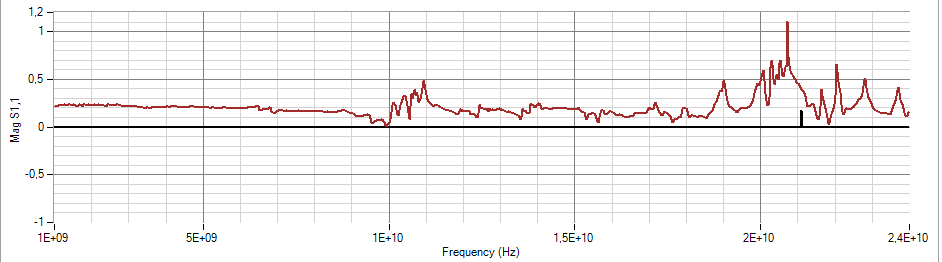
\includegraphics[width=\linewidth]{Fotos/Mediciones/L1_S11.PNG}
	\caption{Short Line S11. Comparación entre los valores ideales (rojo) y medidos (negro).}
\end{figure}

\begin{figure}[hbt!]
	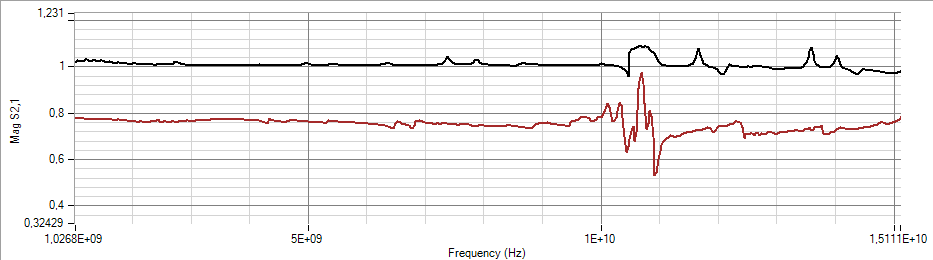
\includegraphics[width=\linewidth]{Fotos/Mediciones/L1_S21.PNG}
	\caption{Short Line S21. Comparación entre los valores ideales (rojo) y medidos (negro).}
\end{figure}

\begin{figure}[hbt!]
	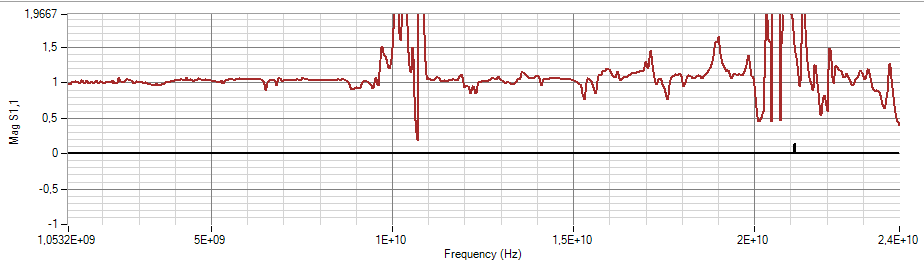
\includegraphics[width=\linewidth]{Fotos/Mediciones/L2_S11.PNG}
	\caption{Long Line S11. Comparación entre los valores ideales (negro) y medidos (rojo).}
\end{figure}

\begin{figure}[hbt!]
	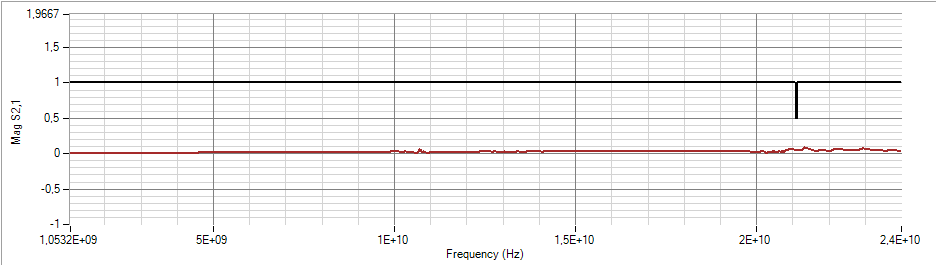
\includegraphics[width=\linewidth]{Fotos/Mediciones/L2_S21.PNG}
	\caption{Long Line S21. Comparación entre los valores ideales (negro) y medidos (rojo).}
\end{figure}

\begin{figure}[hbt!]
	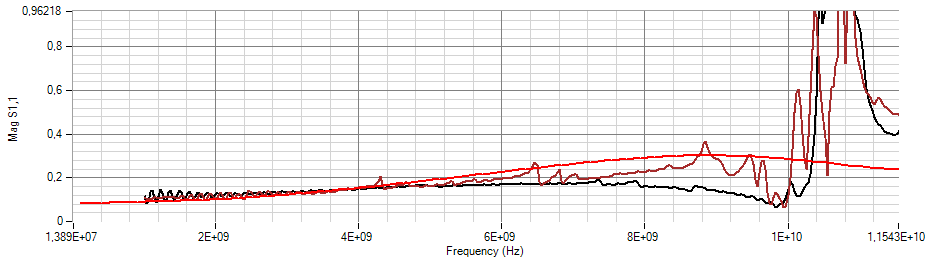
\includegraphics[width=\linewidth]{Fotos/Mediciones/DUT_S11.PNG}
	\caption{DUT S11. Comparación entre los valores ideales (rojo), medido con placa con errores (marrón)
	y finalmente medido y corregido con placa definitiva (negro).}
\end{figure}

\begin{figure}[hbt!]
	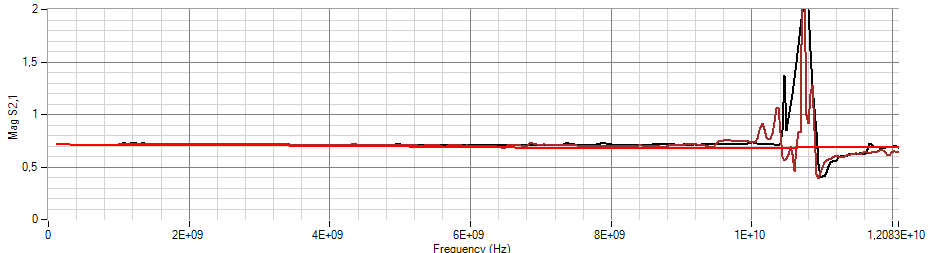
\includegraphics[width=\linewidth]{Fotos/Mediciones/DUT_S21.PNG}
	\caption{DUT S11. Comparación entre los valores ideales (rojo), medido con placa con errores (marrón)
	y finalmente medido y corregido con placa definitiva (negro).}
\end{figure}

\begin{figure}[hbt!]
	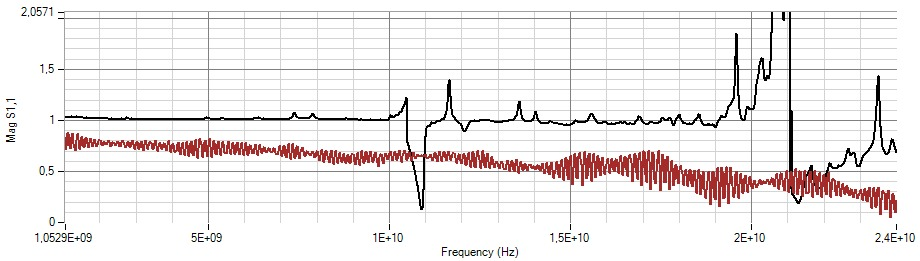
\includegraphics[width=\linewidth]{Fotos/Mediciones/Short_S11.jpeg}
	\caption{Short S11. Comparación entre los valores ideales (negro) y medidos (rojo).}
\end{figure}

\clearpage

\subsection{Otras capturas del proceso de medición}

\begin{figure}[hbt!]
	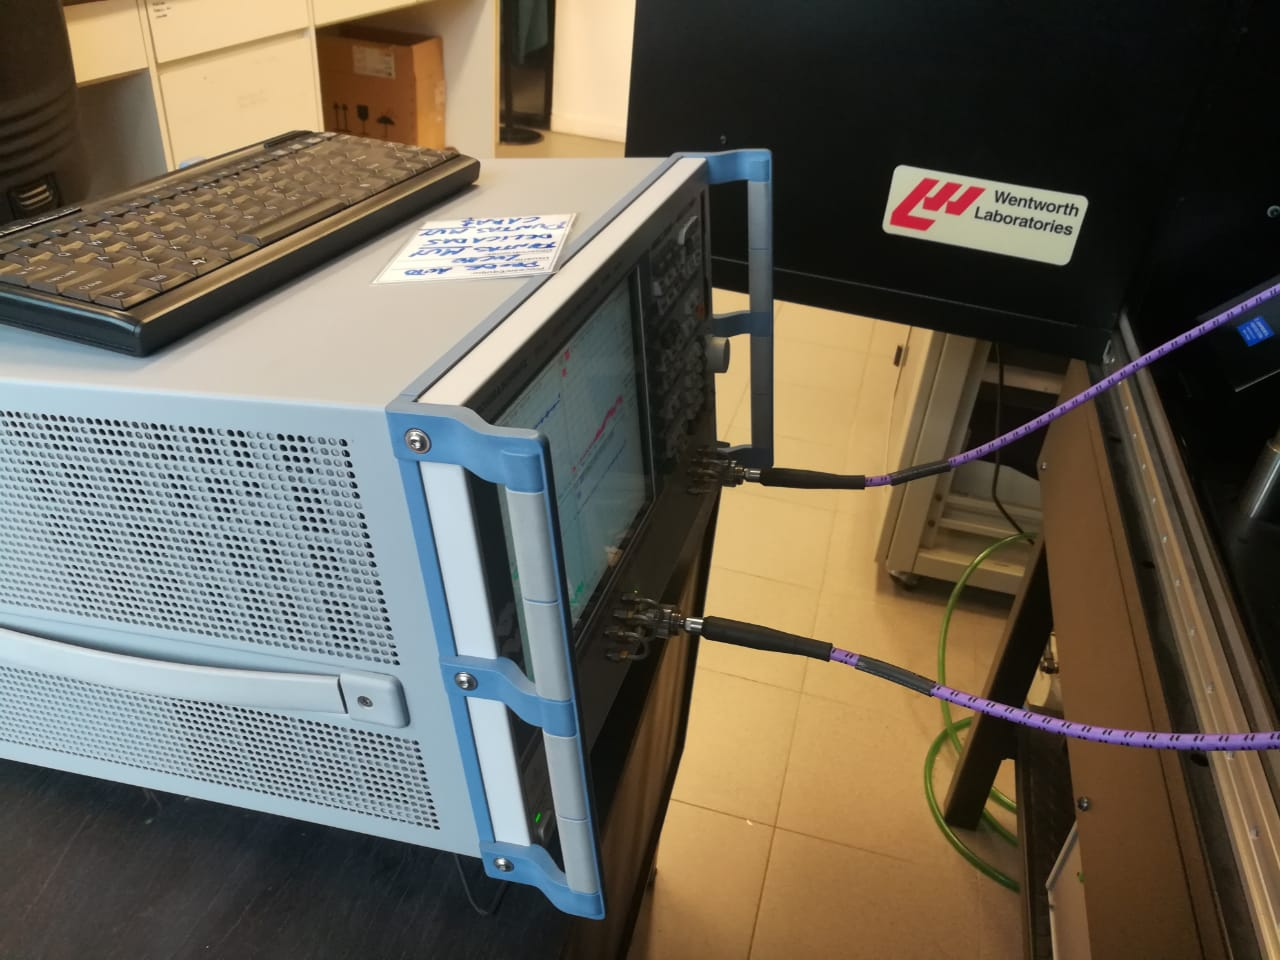
\includegraphics[width=\linewidth]{Fotos/Med_1.jpeg}
	\caption{Rohde \& Schwarz ZVA 24.}
\end{figure}

\begin{figure}[hbt!]
	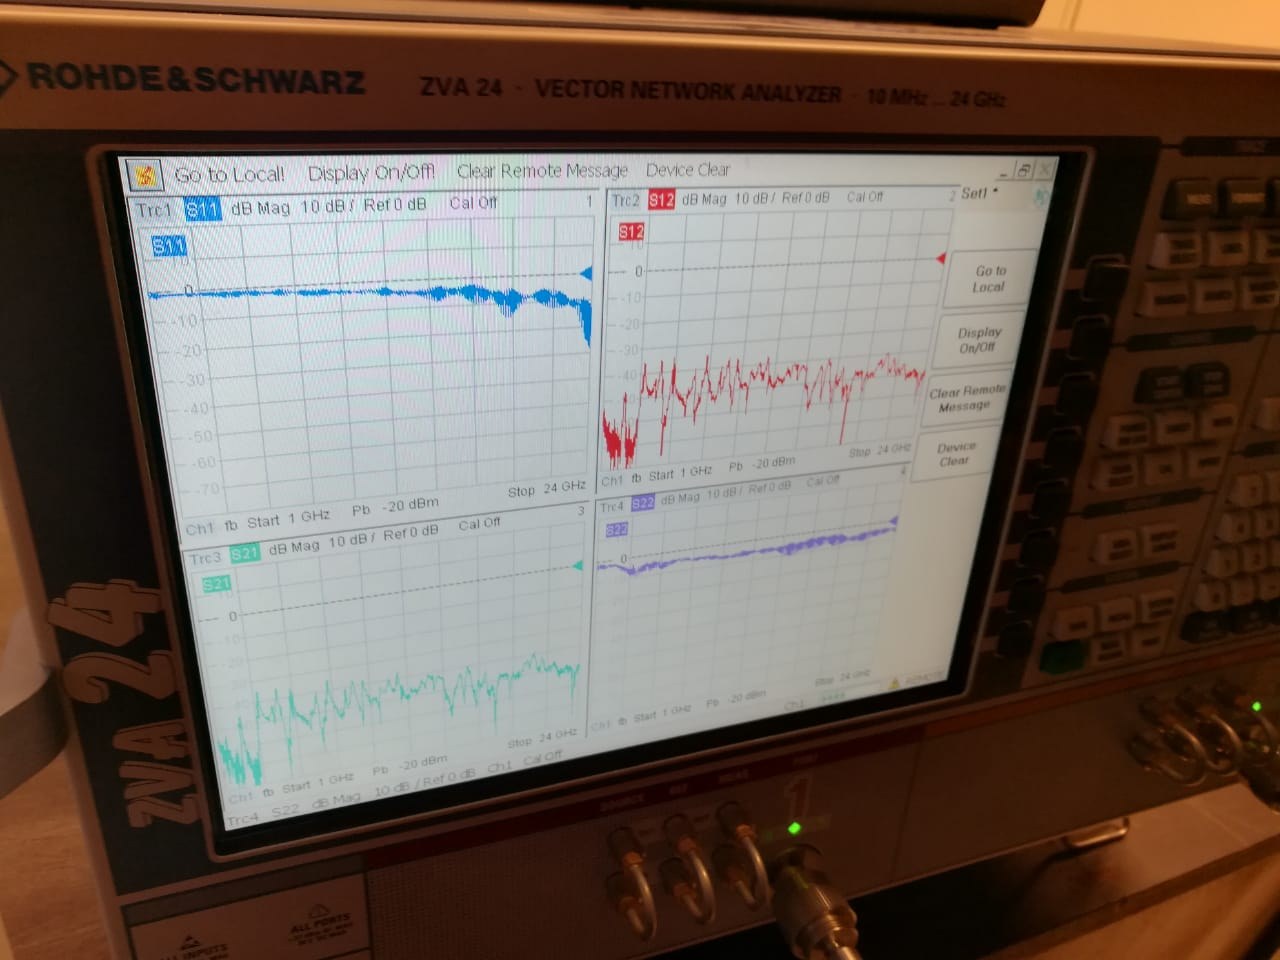
\includegraphics[width=\linewidth]{Fotos/Med_2.jpeg}
	\caption{Proceso de medición.}
\end{figure}

\begin{figure}[hbt!]
	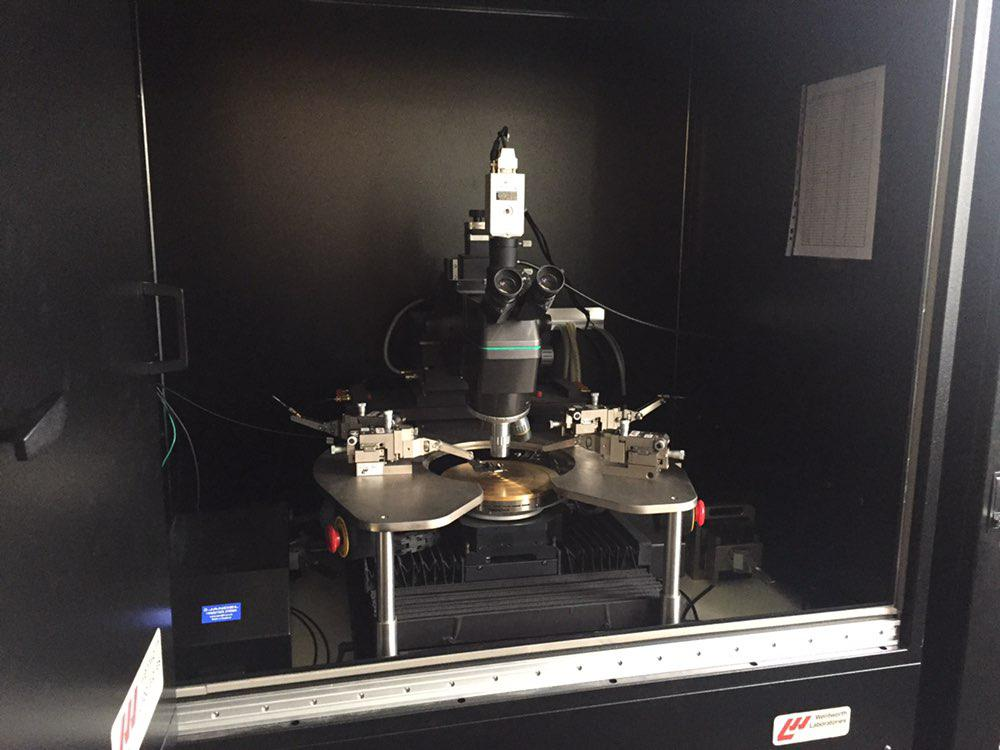
\includegraphics[width=\linewidth]{Fotos/Med_3b.jpg}
	\caption{Estación de medición.}
\end{figure}

\begin{figure}[hbt!]
	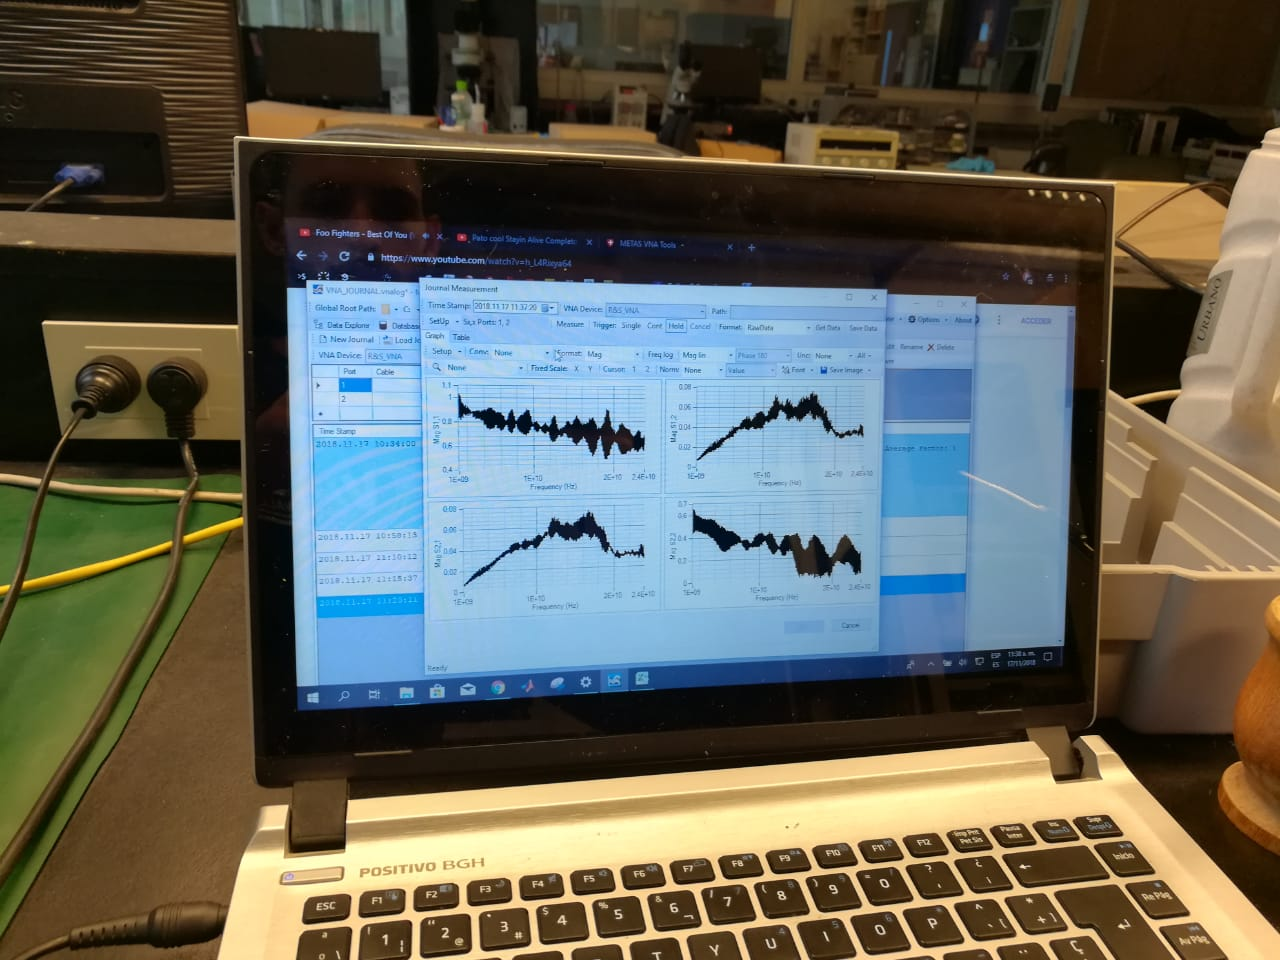
\includegraphics[width=\linewidth]{Fotos/Med_3.jpeg}
	\caption{VNA Tools.}
\end{figure}

\begin{figure}[hbt!]
	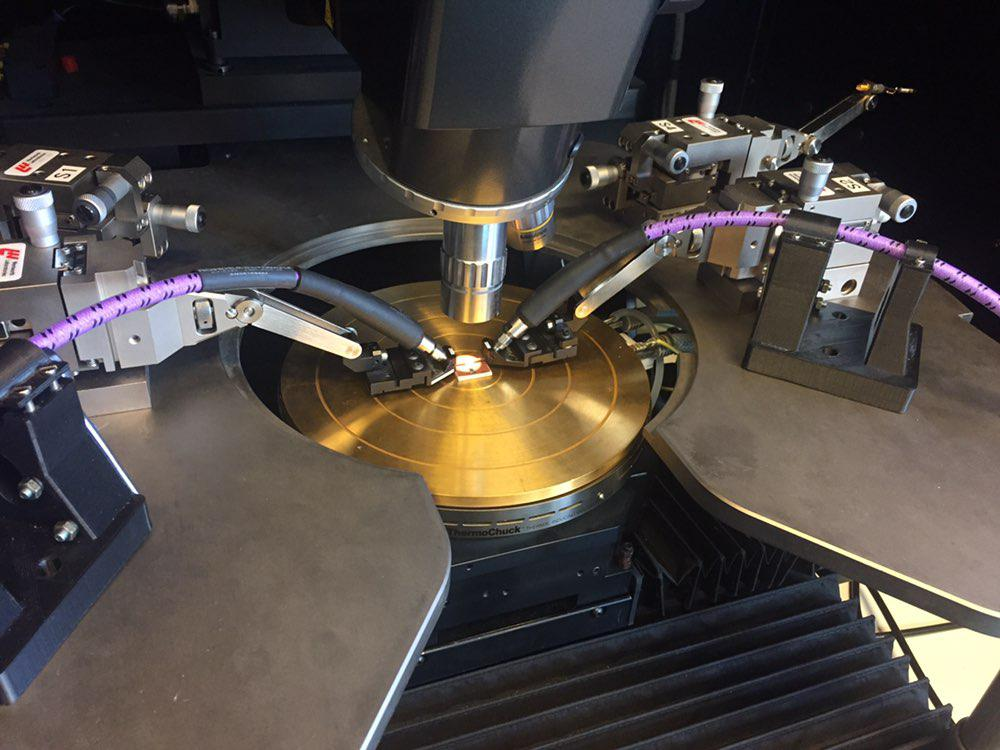
\includegraphics[width=\linewidth]{Fotos/Med_4.jpg}
	\caption{Estación de medición y puntas de prueba.}
\end{figure}

%------------------------------------------------
\section{Inconvenientes y consideraciones}

Presentamos a continuación algunos inconvenientes que se fueron encontrando y
superando a lo largo del proceso.
\begin{itemize}
\item Revisar todos los aspectos e imperfecciones del diseño antes de la impresión de la filmina. Revisar con diversos visores (pdf, imágenes, etc).
\item Minimizar el tamaño de los contactos/pads (llamadas launchers) de cada uno de los patrones (para reducir imperfecciones y mediciones indeseadas).
\item No usar conectores (generalmente SMA) baratos.
\item Utilizar preferentemente un corto-circuito (short) para el patrón Reflect.
\item Tener en cuenta tiempos de entrega, demoras y posibles imprevistos en caso de adquirir
componentes de algún proveedor del exterior.
\item Tener en cuenta desde un principio las características del probe.
\end{itemize}

%------------------------------------------------
\section{Conclusiones}

Nos encontramos con diversas situaciones adversas a lo largo del proyecto, algunas de las cuales estaban
relacionadas con aspectos técnicos y tecnológicos mientras que otras tenían que ver áreas de planifiación, proveedores, etc. La etapa de investigación y diseño pudo completarse sin mayores inconvenientes, teniendo
a tiempo la elección de componentes y diseño de PCB. Los mayores inconvenientes surgieron en la etapa de
fabricación, donde efectivamente nos encontramos con problemas del mundo real (proveedores que no cumplen
con lo solicitado, demoras en entregas, etc). Una vez superados dichos inconvenientes fue un desafío familiarizarse con los instrumentos de medición (VNA y puntas de prueba). Finalmente pudimos verificar en
forma satisfactoria y realizar mediciones sobre el DUT.

%----------------------------------------------------------------------------------------
%	BIBLIOGRAPHY
%----------------------------------------------------------------------------------------

\medskip

\begin{thebibliography}{9}

\bibitem{attenuator}
Analog Devices HMC652LP2E
\\\texttt{https://www.analog.com/media/en/technical-documentation/data-sheets/hmc652lp2-hmc655lp2.pdf}

\bibitem{cpw}
Coplanar waveguide
\\\texttt{https://en.wikipedia.org/wiki/Coplanar\_waveguide}

\bibitem{rogers}
Rogers RO3210
\\\texttt{https://www.rogerscorp.com/documents/725/acs/RO3200-Laminate-Data-Sheet-RO3203-RO3206-RO3210.pdf}

\bibitem{txline}
TX Line Software
\\\texttt{https://www.awrcorp.com/products/additional-products/tx-line-transmission-line-calculator}

\bibitem{engcrit}
TRL Calibration Blog
\\\texttt{https://www.microwaves101.com/encyclopedias/trl-calibration}

\bibitem{vna}
Rohde \& Schwarz ZVA 24
\\\texttt{https://www.rohde-schwarz.com/us/product/zva-productstartpage\_63493-9660.html}

\bibitem{probe}
PICOPROBE Model 40A
\\\texttt{http://www.ggb.com/40a.html}

\bibitem{metas}
Metas VNA Tools
\\\texttt{https://www.metas.ch/metas/en/home/fabe/hochfrequenz/vna-tools.html}

\end{thebibliography}
%----------------------------------------------------------------------------------------

\end{document}
